\section{随机加法器和积分器}

在了解了如何通过简单门电路轻松实现求反和乘法之后，人们或许会想当然地认为类似的门电路也可用来实现加法. 然而事实并非如此，必须引入随机逻辑元件来对两个随机序列所表示的量进行求和. 例如，考虑表示 (i) 中的两个随机序列，一个表示最大正量因此始终为 ON，另一个表示最大负量因此始终为 OFF. 这两个量之和为零，其表示是一个 ON 和 OFF 概率相等的随机序列. 无法从具有恒定输入的确定性门电路获得概率性输出，因此必须在随机计算机的求和门电路中内置随机行为.

随机加法器可被视为一种开关，它在时钟脉冲时随机选择一条输入线并将其连接到输出端. 输出线则表示输入线所表示的量的和，根据选择特定输入线的概率进行加权. 随机选择由内部生成的随机序列执行，这些序列通过采样由高带宽噪声源触发的触发器，或从中央伪随机移位寄存器的延迟序列获得. 称这些序列为「数字噪声」.

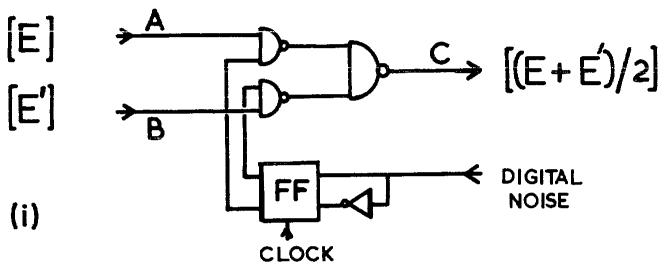
\includegraphics[width=0.6\textwidth, height=7cm, keepaspectratio]{images/5dc94beb4b8df8ffaa7d0969fa68d04c38fcfc80f4ba37c1f9038e19a6ebcd10.jpg}

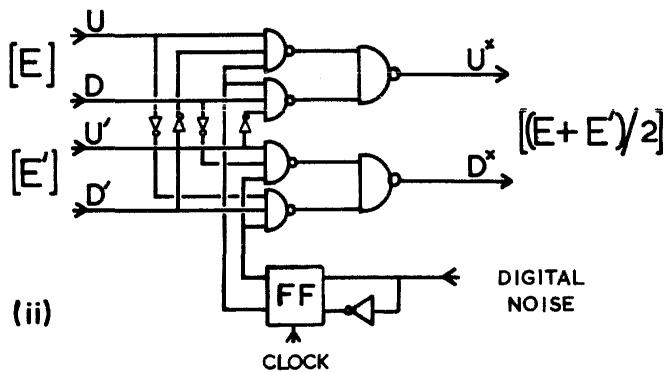
\includegraphics[width=0.6\textwidth, height=7cm, keepaspectratio]{images/bbed31d4771fbde4344e3774419967d9fc2a2d9dec06eb85f04836fb0862bd0f.jpg}\\
Figure 5---随机加法器

表示 (i) 和 (ii) 中用于两个输入的随机加法器分别如图 5(i) 和 5(ii) 所示. 图 5(ii) 中输入之间的交叉耦合降低了输出的方差. 检查图 5 中门电路的输入和输出概率之间的关系，可确认确实执行了加法. 对于 5(i)，假设数字噪声对称分布：

\[
\mathbf {p} (\mathrm {C}) = \frac {1}{2} \mathbf {p} (\mathrm {A}) + \frac {1}{2} \mathbf {p} (\mathrm {B}) \tag {15}
\]

因此，根据公式 (10) 和 (11)：---

\[
\mathbf {p} (\mathbf {C}) = \frac {1}{2} \left(\frac {1}{2} \left(\mathrm {E} + \mathrm {E} ^ {\prime}\right)\right) / \mathrm {V} + \frac {1}{2} \tag {16}
\]

这是 $\mathbf{E}$ 和 $\mathbf{E}^{\prime}$ 的归一化求和. 将公式 (4) 代入以下关系式，可为 5(ii) 获得类似结果：

\[
\begin{array}{l} p (U ^ {x}) = \frac {1}{2} p (U) (1 - p (D ^ {\prime})) + \frac {1}{2} p (U ^ {\prime}) \\ (1 - \mathbf {p} (D)) \tag {17} \\ \end{array}
\]

\[
\begin{array}{l} p \left(\mathrm {D} ^ {\mathrm {x}}\right) = 1 / 2 p (\mathrm {D}) (1 - p \left(\mathrm {U} ^ {\prime}\right)) + 1 / 2 p \left(\mathrm {D} ^ {\prime}\right) \\ (1 - p (U)) \tag {18} \\ \end{array}
\]

随机积分器、ADDIE 和接口

随机计算机中的基本积分器是可逆计数器---若它有 $\mathbf{N} + 1$ 个状态，则当其处于第 k 个状态时，积分的值为：

\[
f = (2 k / N - 1) V \tag {19}
\]

若要在进一步的计算中使用这个量，必须将其作为随机序列提供，这可通过将计数器中的二进制数与均匀分布的数字随机数（从中央伪随机移位寄存器或采样循环计数器获得）进行比较来生成. 在表示 (i) 中，若存储计数大于随机数，则积分器输出线为 ON. 在表示 (ii) 中，存储计数被视为二进制补码表示的数，其幅度与随机数比较，其符号与比较结果一起决定 UP 或 DOWN 输出线应为 ON.

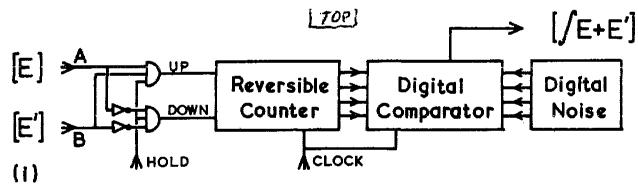
\includegraphics[width=0.6\textwidth, height=7cm, keepaspectratio]{images/007a2e69d1cdef90fea0e84ae3f7f572dd8e39f1a4ab896936ec0d15e7299444.jpg}

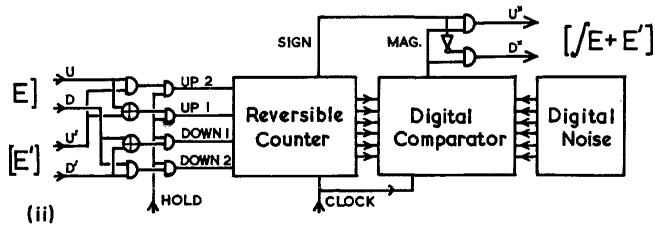
\includegraphics[width=0.6\textwidth, height=7cm, keepaspectratio]{images/16ec18facc1380b8aa3b7486b50e51a35cfe61959404adde710f746e5c26117d.jpg}\\
Figure 6---随机积分器

图 6 显示了每种表示的两个输入随机积分器，其输出线如上所述，并在计数器输入端设置门电路以形成输入线所表示量的和（不需要随机求和，因为用于表示和的线数大于用于表示每个输入的线数）. 积分器输入端的 HOLD 线决定它们处于积分模式还是保持模式，并且

正常的积分器符号用于整体设备，如图 7 所示.

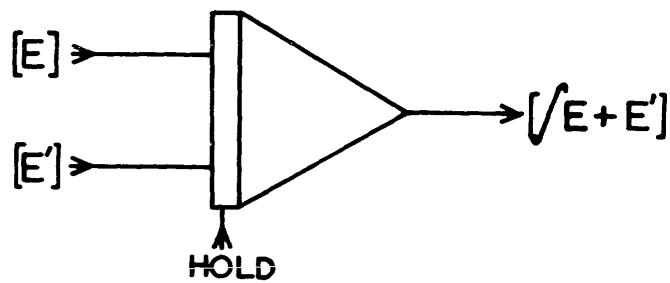
\includegraphics[width=0.6\textwidth, height=7cm, keepaspectratio]{images/75a79ae91e0524d8a4a085913776e7eb6366e36494880280cd89973d641fcbec.jpg}\\
Figure 7---积分器符号

检查每个时钟脉冲时计数器的预期增量 $\delta$，可确认确实执行了积分. 对于 6(i)：

\[
\begin{array}{l} \delta = \frac {2 \mathrm {V}}{\mathrm {N}} [ \mathrm {p} (\mathrm {A}) \mathrm {p} (\mathrm {B}) - (1 - \mathrm {p} (\mathrm {A}) (1 - \mathrm {p} (\mathrm {B})) ] (20) \\ = \left(\mathrm {E} + \mathrm {E} ^ {\prime}\right) / \mathrm {N} (21) \\ \end{array}
\]

代入公式 (10) 和 (11)，这等效于一个具有时间常数的积分器：

\[
\mathrm {T} = \mathrm {N} / \mathrm {f} \tag {22}
\]

其中 $f$ 是时钟频率. 将公式 (4) 代入以下关系式，可为 6(ii) 获得类似结果：

\[
\begin{array}{l} \delta = \frac {2 \mathrm {V}}{\mathrm {N}} [ 2 \mathrm {p} (\mathrm {U}) \mathrm {p} (\mathrm {U} ^ {\prime}) + \mathrm {p} (\mathrm {U}) (1 - \mathrm {p} (\mathrm {U} ^ {\prime})) + \mathrm {p} (\mathrm {U} ^ {\prime}) \\ (1 - p (U)) - 2 p (D) p \left(D ^ {\prime}\right) - p (D) (1 - p \left(D ^ {\prime}\right)) \\ - p (D ^ {\prime}) (1 - p (D)) ] (23) \\ = \frac {2 V}{N} [ p (U) - p (D) + p \left(U ^ {\prime}\right) - p \left(D ^ {\prime}\right) ] (24) \\ = 2 \left(\mathrm {E} + \mathrm {E} ^ {\prime}\right) / \mathrm {N} (25) \\ \end{array}
\]

这等效于一个具有时间常数的积分：

\[
\mathrm {T} = \mathrm {N} / 2 \mathrm {f} \tag {26}
\]

其中 $f$ 是时钟频率.

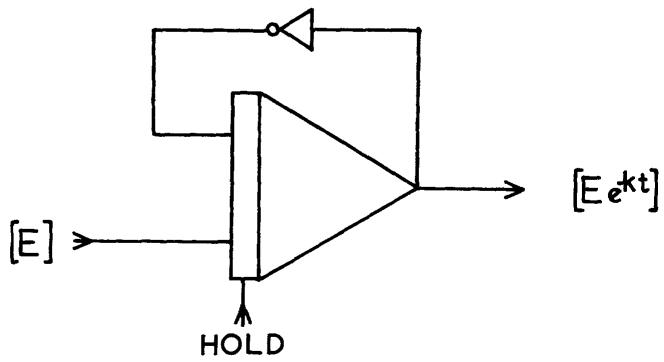
\includegraphics[width=0.6\textwidth, height=7cm, keepaspectratio]{images/0cdd3c8d1eaae3776bcc0f46af2de49d369be1891bdabfe0bafb2233add619e1.jpg}\\
Figure 8-ADDIE

图 8 所示的具有单位反馈的积分器称为 ADDIE，它执行对其输入所表示的量进行指数平均的重要功能. 就所表示的量而言，它可以被视为传递函数：$1 / (s + 1)$. 就随机序列而言

可证，存储器中的分数计数趋于输入线在时钟脉冲时为 ON 的概率的无偏估计（对于如图 8 所示连接的图 6(i) 积分器）. 即，对于处于 $k^{\prime}$ 状态的 $\mathbf{N} + 1$ 状态存储器：

\[
\hat {\mathbf {p}} (\text {I N P U T} = \mathrm {O N}) = \mathrm {k} / \mathrm {N} \tag {27}
\]

估计时间为 N 个时钟脉冲数量级，最终方差为：

\[
\sigma^ {2} (\hat {\mathfrak {p}}) = \mathrm {p} (1 - \mathrm {p}) / \mathrm {N} \tag {28}
\]

因此，随机计算机中由概率线性表示的任何量均可通过使用具有足够多状态的 ADDIE 以任意所需精度读出，但状态越多，平滑的时间常数越长，计算机的带宽越低. 由于积分器中计数的分布是二项分布，因此对于大 N 近似正态分布，随机计算机内的变量可被视为被 Gaussian 噪声退化，其功率随计算机所需带宽成比例增加.

积分器或 ADDIE 构成随机计算机的自然输出接口. HOLD 线为 OFF 的积分器也构成数字或模拟数据的输入接口，因为可以直接将二进制数传送到计数器中以生成随机输出序列，并且可以通过将模拟量与由驱动数模转换器的循环计数器生成的标准斜坡进行比较来将其转换为二进制形式. 类似地，若与乘法器耦合，积分器可用于保持常数，从而充当「电位器」. 可通过在存储计数和随机输出之间施加适当的非线性关系来实现任意函数关系. 例如，一个积分器当其输出在计数值等于或高于中值时为 ON，在低于中值时为 OFF [表示 (i) 中]，近似于开关函数.

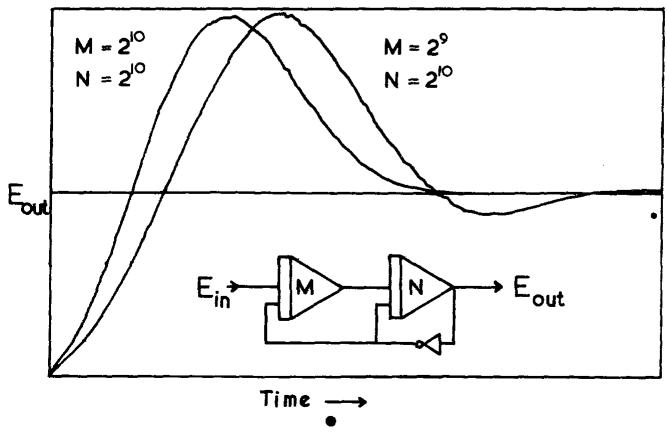
\includegraphics[width=0.6\textwidth, height=7cm, keepaspectratio]{images/ed44eb7f2d5c2d711785ea2583ca50f72f6b7b5057c9faad71f2c99fcd1d2e5f.jpg}\\
Figure 9---随机二阶传递函数---对位置和速度单位阶跃的响应

通过将积分器级联连接并设置适当的反馈回路，可以实现比 ADDIE 更高阶的平滑. 图 9 的插图显示了使用表示 (i) 中两个随机积分器的稳定二阶随机传递函数. 若第一个积分器有 $\mathbf{M} + 1$ 个状态，第二个有 $\mathbf{N} + 1$ 个状态，则实现的变换为：

\[
\frac {\mathrm {M N}}{\mathrm {f} ^ {2}} \mathrm {E} _ {\text {o u t}} + \frac {\mathrm {M}}{\mathrm {f}} \mathrm {E} _ {\text {o u t}} + \mathrm {E} _ {\text {o u t}} = \mathrm {E} _ {\text {i n}} \tag {29}
\]

其中 $f$ 是时钟频率. 因此无阻尼自然频率为：

\[
\mathrm {f} _ {\mathrm {n}} = \frac {\mathrm {f}}{2 \Pi (\mathrm {M N}) ^ {1 / 2}} \tag {30}
\]

阻尼比为：

\[
\Sigma = 1 / 2 (\mathrm {M} / \mathrm {N}) ^ {1 / 2} \tag {31}
\]

对位置和速度单位阶跃的响应如图 9 所示，对应两种条件：$\mathbf{M} = 2^{10}$，$\mathbf{N} = 2^{10}$ 和 $\mathbf{M} = 2^{9}$，$\mathbf{N} = 2^{10}$. 这些是在 STL 的 Mark I 随机计算机上获得的.
